
\section{Contributions of this study}

\begin{enumerate}

\item This thesis proposes a meta-learning algorithm that adopts a unique approach of utilizing principles that counterbalance each other - boosting and bagging. Bagging generates more robust models at the expense of bias and boosting transforms weak learners into stronger ones. Boosting a traditional forest of trees did not give competitive results as the learners it created were not diverse enough. BXT in essence tries to induce diversity in its outputs at the expense of accuracy by making them less deterministic (random splits for a random choice of features). This makes the extremely random tree learner a sub-optimal stand alone model which very often is less competitive to the traditional random forest \cite{xrf}. However, the randomization trick makes the extremely random tree a good choice for boosting as it is in a position to harness the weight updates in boosting for several stages until it saturates. This thesis demonstrates the effectiveness of a boosted tree ensemble versus the traditional approach in HEP of boosting single decision trees. 

\item This thesis provides a systematic study of a challenging classification problem presented in the ATLAS Higgs dataset from the perspective of a machine learner. By providing a model which achieves a competitive AMS score it sets an effective performance threshold achievable by using the basic tree learner in an innovative re-incarnation. It also provides a threshold against which more sophisticated models can be rated and compared. This is in keeping with the Occam's razor approach which states simpler models should be preferred over more complex ones if their performances are similar. In conducting this study it has come to light that some of the solutions proposed for achieving high scores on this dataset were powerful but superfluous \cite{melis}. Similar scores are achievable using much simpler architectures, one such has been described in this thesis. 

\end{enumerate}

In order to put into perspective the model developed in this thesis, the fig. \ref{win} shows the leading solutions to the ATLAS Higgs dataset. 

\begin{figure}
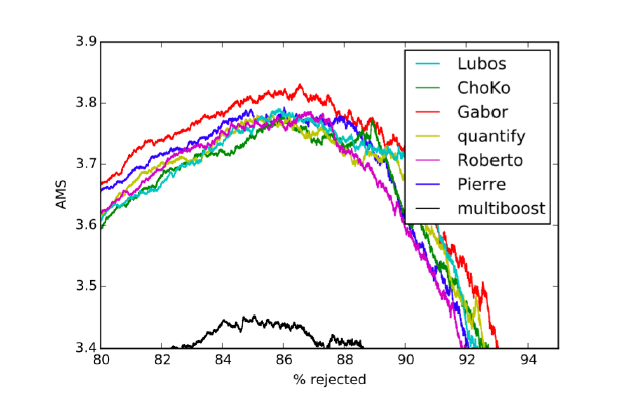
\includegraphics[scale=0.6]{images/WinningAMS.png}
\caption{Leading Solutions to the Kaggle ATLAS Higgs machine learning challenge. The challenge used the same dataset as the one used in this thesis. Adapted from \cite{postRM}.}
\label{win}
\end{figure}   

\begin{figure}
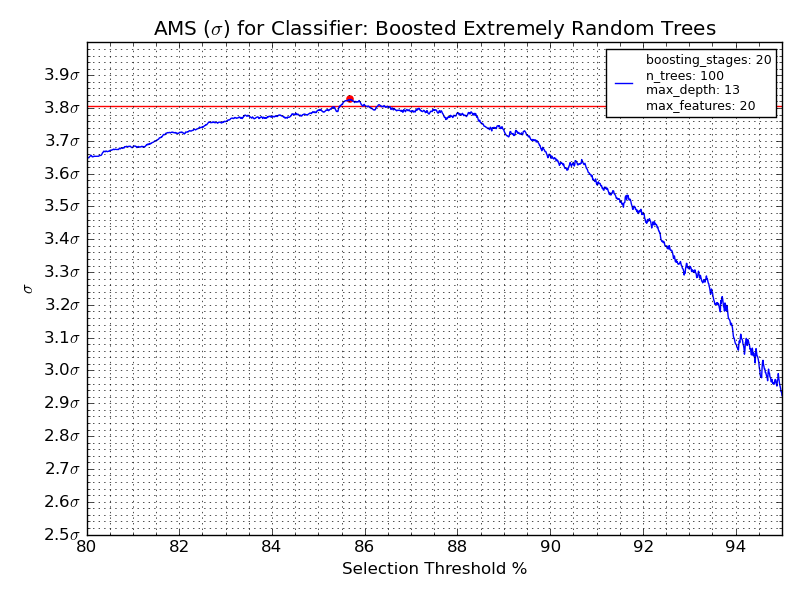
\includegraphics[scale=0.6]{images/AMS_Curve_BXT_opt.png}
\caption{BXT solution to the ATLAS Higgs dataset.}
\end{figure}

\section{Related / Future Work}

As any study does, this study also creates some new questions which could be interesting for the HEP community of machine learners at large. They could form the basis of future or related research trajectories. 

\begin{itemize}
\item The work in this thesis provides an innovative way to use a primitive learner like a tree for classification in an extremely challenging setting. The work does not explore changing the way a primitive binary tree learns. One of the fundamental building blocks of tree learning is the splitting criterion, and majority of the studies that focus on applications of tree learning use axis-parallel linear splits .i.e they split on a single feature at each node. Geometrically, these univariate splits at each node can be thought of generating space partitioning hyperplanes parallel to the feature axis. Splitting criterion that generate oblique splits by using a linear combination of attribute values, could perform very differently to the primitive tree with linear splits. They generate polygonal partitions in feature space instead of rectangular ones.  There is very little research on such trees and hardly any software packages offer implement construction of such trees \cite{oblique}. 
\item Bagging and boosting can be combined in various ways, the approach in this thesis using primitive trees is one example, and is in no way the final word on the topic \cite{combining, combining2}. 
\item Deriving theoretical performance bounds on learning from primitive learners like binary trees. As we have seen, additional classification power can be extracted from trees by using enough of them and re-combining them. How far they can be stretched in the context of a specific problem is established through experimentation, by looking for convergence in one or more performance criteria. The analysis present in this thesis is a coarse-grained approach to optimization in the presence of a non-standard performance metric, but can we do better than optimization by hand? 
\end{itemize}

Boosting uses an internal bifurcation procedure to split data into ones that were misclassified and others, in this way it passes information about learning in one stage to the next. The samples that are misclassified in early stages are the ones that lie in the most overlapping regions of the feature space. It is possible to enrich data with this meta-information before training commences or in between the boosting stages. Meta information that captures a spatial attribute of the dataset like degree of overlap for each data point could add classification power to trees which are rule based learners and do not capture this information about the geometric structure of the dataset. This would be a way to combine the power of rule based and distance based learning.  

\begin{sidewaysfigure}
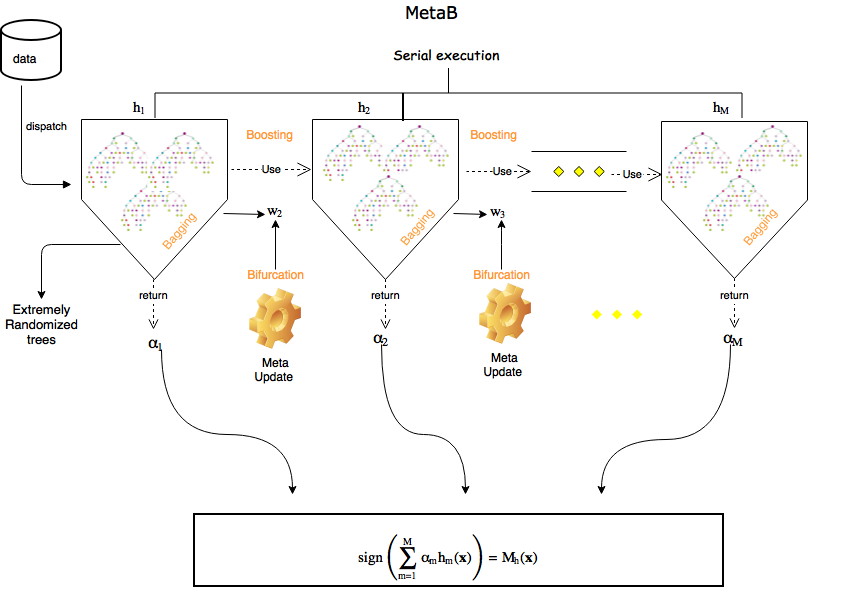
\includegraphics[scale=0.75]{images/metab.png}
\caption{Architecture of a proposed algorithm that could combine three meta learning techniques - bagging, boosting and bifurcation in a unified framework}
\end{sidewaysfigure}

\section{Concluding Remarks}

\subsection{On Methodology}

The methodology used in this thesis provides a unified framework for two of the most successful ensemble learning techniques - boosting and bagging. In doing so, it shows that it is possible to achieve performance gains from a carefully fine-tuned combination of the two. The randomization trick used in the BXT model is able to achieve greater diversity in tree outputs while benefiting from boosting for longer than a traditional tree or a random forest. I believe it is this nested combination of randomization within boosting that provides a performance edge in this particular dataset. This is an effective technique to use in the presence of data that is overlapping and ambiguous.

\subsection{On the ATLAS Higgs dataset}

The methodology presented in this thesis presents one approach for tackling the challenges presented in the ATLAS Higgs dataset. The approach suggested here is unique in its study of the problem as it does not rely on the raw classification power of the base learner, rather it relies on the power of randomization and repetition to improve learning in very rudimentary structures like binary trees. This raises the question as to whether enough trees can achieve the same accuracy provided through neural networks which are currently slated to be the most successful learners in this domain. It also brings up a more general question about the links between \textit{learning} and \textit{randomization} in non-linear settings. 

\subsection{On the scientific validity of inference}
Any contemporary science abounds in questions of statistical nature. The current era of science is defined by experiments where the process of scientific discovery hinges upon the correct analysis of scientific data. This is largely because of the ubiquity of data and open access to it. This has also led to the proliferation of modern learning techniques like deep neural networks. The issues involved in designing good standards for scientific inference are challenging and can be thought of as techniques of  meta-analyses (analyses of analyses). Performance assessment is not standardised but is tied to the problem being solved, this creates further challenges. In the Higgs dataset dealt with in this thesis it was not enough to produce classifiers with high accuracy. In fact, that was not the assessment criterion, the assessment criterion was a narrowly defined significance metric, the AMS $\sigma$. What counts as good performance and how to design performance metrics for learning algorithms that cover a vast array of problems? This is a meta field of research which attracts relatively less interest from scientists and practitioners. This is perhaps due to the attraction of objective rules (like a $p$ value $\leq 0.01$ makes for a very significant result rather than $p$ value $\leq 0.03$) and aversion for subjective interpretation. The usage of the Fisherian $p$ value has not changed in the last century and we continue to rely on it in answering questions of great scientific importance in physics, genetics and medicine. The question about whether the $H \rightarrow \tau^{+}\tau^{-}$ decay will ever reach $5\sigma$ is still an open one. With learning techniques rapidly growing in power and sophistication, there are hints that it could. However, even if it does, what does that really mean? 